\documentclass{article}
\usepackage[utf8]{inputenc}
\usepackage{titling} % package per il titolo
\usepackage{graphicx}
\usepackage{hyperref} % package per i collegamenti cliccabili
\usepackage{listings} % package per inserire il codice
\usepackage{xcolor} % package per i colori
\usepackage{float} % usato per le immagini \begin{figure}[H] per mettere la H che evita che le immagini vadano in pagine successive
\usepackage{amsmath}
\usepackage{parskip}
\usepackage[inner=1cm,outer=1cm,bottom=1cm,top=1cm]{geometry}

\definecolor{shellGreen}{RGB}{19,193,106}
\definecolor{backcolor}{rgb}{0.95,0.95,0.92}
\definecolor{mateBlack}{RGB}{45,45,50}
\definecolor{comment}{rgb}{0.1,0.6,0.2}
\definecolor{codegray}{rgb}{0.5,0.5,0.5}

% Definisce i colori per il codice in VHDL
\lstdefinestyle{vhdl}{
    language=vhdl,
    frame=single,
    basicstyle=\scriptsize,
    breaklines=true,
    captionpos=b,
    keepspaces=true,
    backgroundcolor=\color{backcolor},
    keywordstyle=[1]\color{blue}\bf,
    keywordstyle=[2]\color{red}\bf,
    keywordstyle=[3]\color{cyan!50}\bf,
    stringstyle=\color{orange},
    commentstyle=\color{comment},
    tabsize=2,
    numbers=left,
    showspaces=false,
    showstringspaces=false,
    showtabs=false,
    moredelim=[s][\textcolor{green}]{component}{is},
    morekeywords=[1]{
        library, use ,all,entty,is,port,in,out,end,architecture,of, body,
        function, variable, begin,and,or,Not,downto,ALL, signal, process, if,
        else, elsif, case, when, then, range, to, component, type, with, select,
        others, constant, inout, buffer, map, true, false, array, subtype, wait,
        wait for, generic, =, <, >, <=, >=, =>,
    },
    alsoletter={=, <, >},
    morekeywords=[2]{
            STD_LOGIC_VECTOR,STD_LOGIC,IEEE,STD_LOGIC_1164, work, local, real,
            math_real, time, NUMERIC_STD,STD_LOGIC_ARITH,STD_LOGIC_UNSIGNED,
            std_logic_vectr, std_logic, ieee, numeric_std, std_ulogic,
            std_logic_1164, natural, bit, bit_vector, signed, unsigned,
            boolean, integer
    },
    morekeywords=[3]{rising_edge, falling_edge, resize, to_signed, to_unsigned},
    morecomment=[l]{--},
    morecomment=[s][\color{orange}]{'}{'},
    numbers=left,
}


\lstset{style=vhdl}
\renewcommand{\lstlistingname}{Code} % cambia il nome per le caption da "Listing" a "Code"

\pagestyle{empty}

\title{\huge Documentazione}
\author{
\Large \textbf{Matteo Battilana} Numero Matricola \\
\Large \textbf{Salvatore Gabriele La Greca} s281589 \\
\Large \textbf{Giovanni Pollo} s290136}
\date{}
\renewcommand\maketitlehooka{
  \begin{center}
    
\includegraphics[width=0.8 \textwidth]{Immagini/Logo_Polito.jpg} % Dimensioni per l'immagine
  \end{center}
}



%%%%%%%%%%%%%%%%%%%% Start of the Document %%%%%%%%%%%%%%%%%%%%

\begin{document}

\begin{titlepage}
  \centering
  \vspace{2px}
\end{titlepage}
\maketitle
\thispagestyle{empty}

\newpage

\tableofcontents

\newpage

\section{Register File}

This section will be divided into subsections in which we describe single components.

\subsection{Decoder}

This block receives as input the \emph{write address} on \textbf{NBIT\_ADD} bits and outputs \(\mathbf{2^{NBIT\_ADD} - 1} \) bits. It has the utility of converting the address of the register at which we need to write into its enable signal. 

The idea is that if the input is \(0b00010\) the output will be \(0b00000000000000000000000000000100\). In fact if the input is decimal 2, it means that we need to write the second register of the \emph{GLOBAL} block. In terms of enable it can be translated by having the bit with index 2 at one. In fact in the output we see that the it with index 2 has value 1, while the others are all 0. 

The output is divided (in the schematic) in order to represent the group of bits. In particular we have that: 
\begin{itemize}
    \item M - 1 DOWNTO 0: bits associated to the \emph{GLOBAL} register
    \item M + N - 1 DOWNTO M: bits associated to the \emph{IN} register
    \item M + 2N - 1 DOWNTO M + N: bits associated to the \emph{LOCAL} register
    \item M + 3N - 1 DOWNTO M + 2N: bits associated to the \emph{OUT} register
\end{itemize}

On the top of the schematic (\autoref{decoder}) we can see an AND logic port between \emph{ENABLE} and \emph{WR} signals. If both \emph{ENABLE} and \emph{WR} are 1, it means that our register need to work. In fact, the output of the dedocer is anded with 1 and so we maintain the value. Otherwise, if one signal between \emph{ENABLE} and \emph{WR} is 0, the output will be 0 and so the AND with the output of the \emph{decoder} will return all 0. 

This signal goes into the \emph{connection matrix}, which is the next block described. 

\begin{figure}[ht]
    \centering
    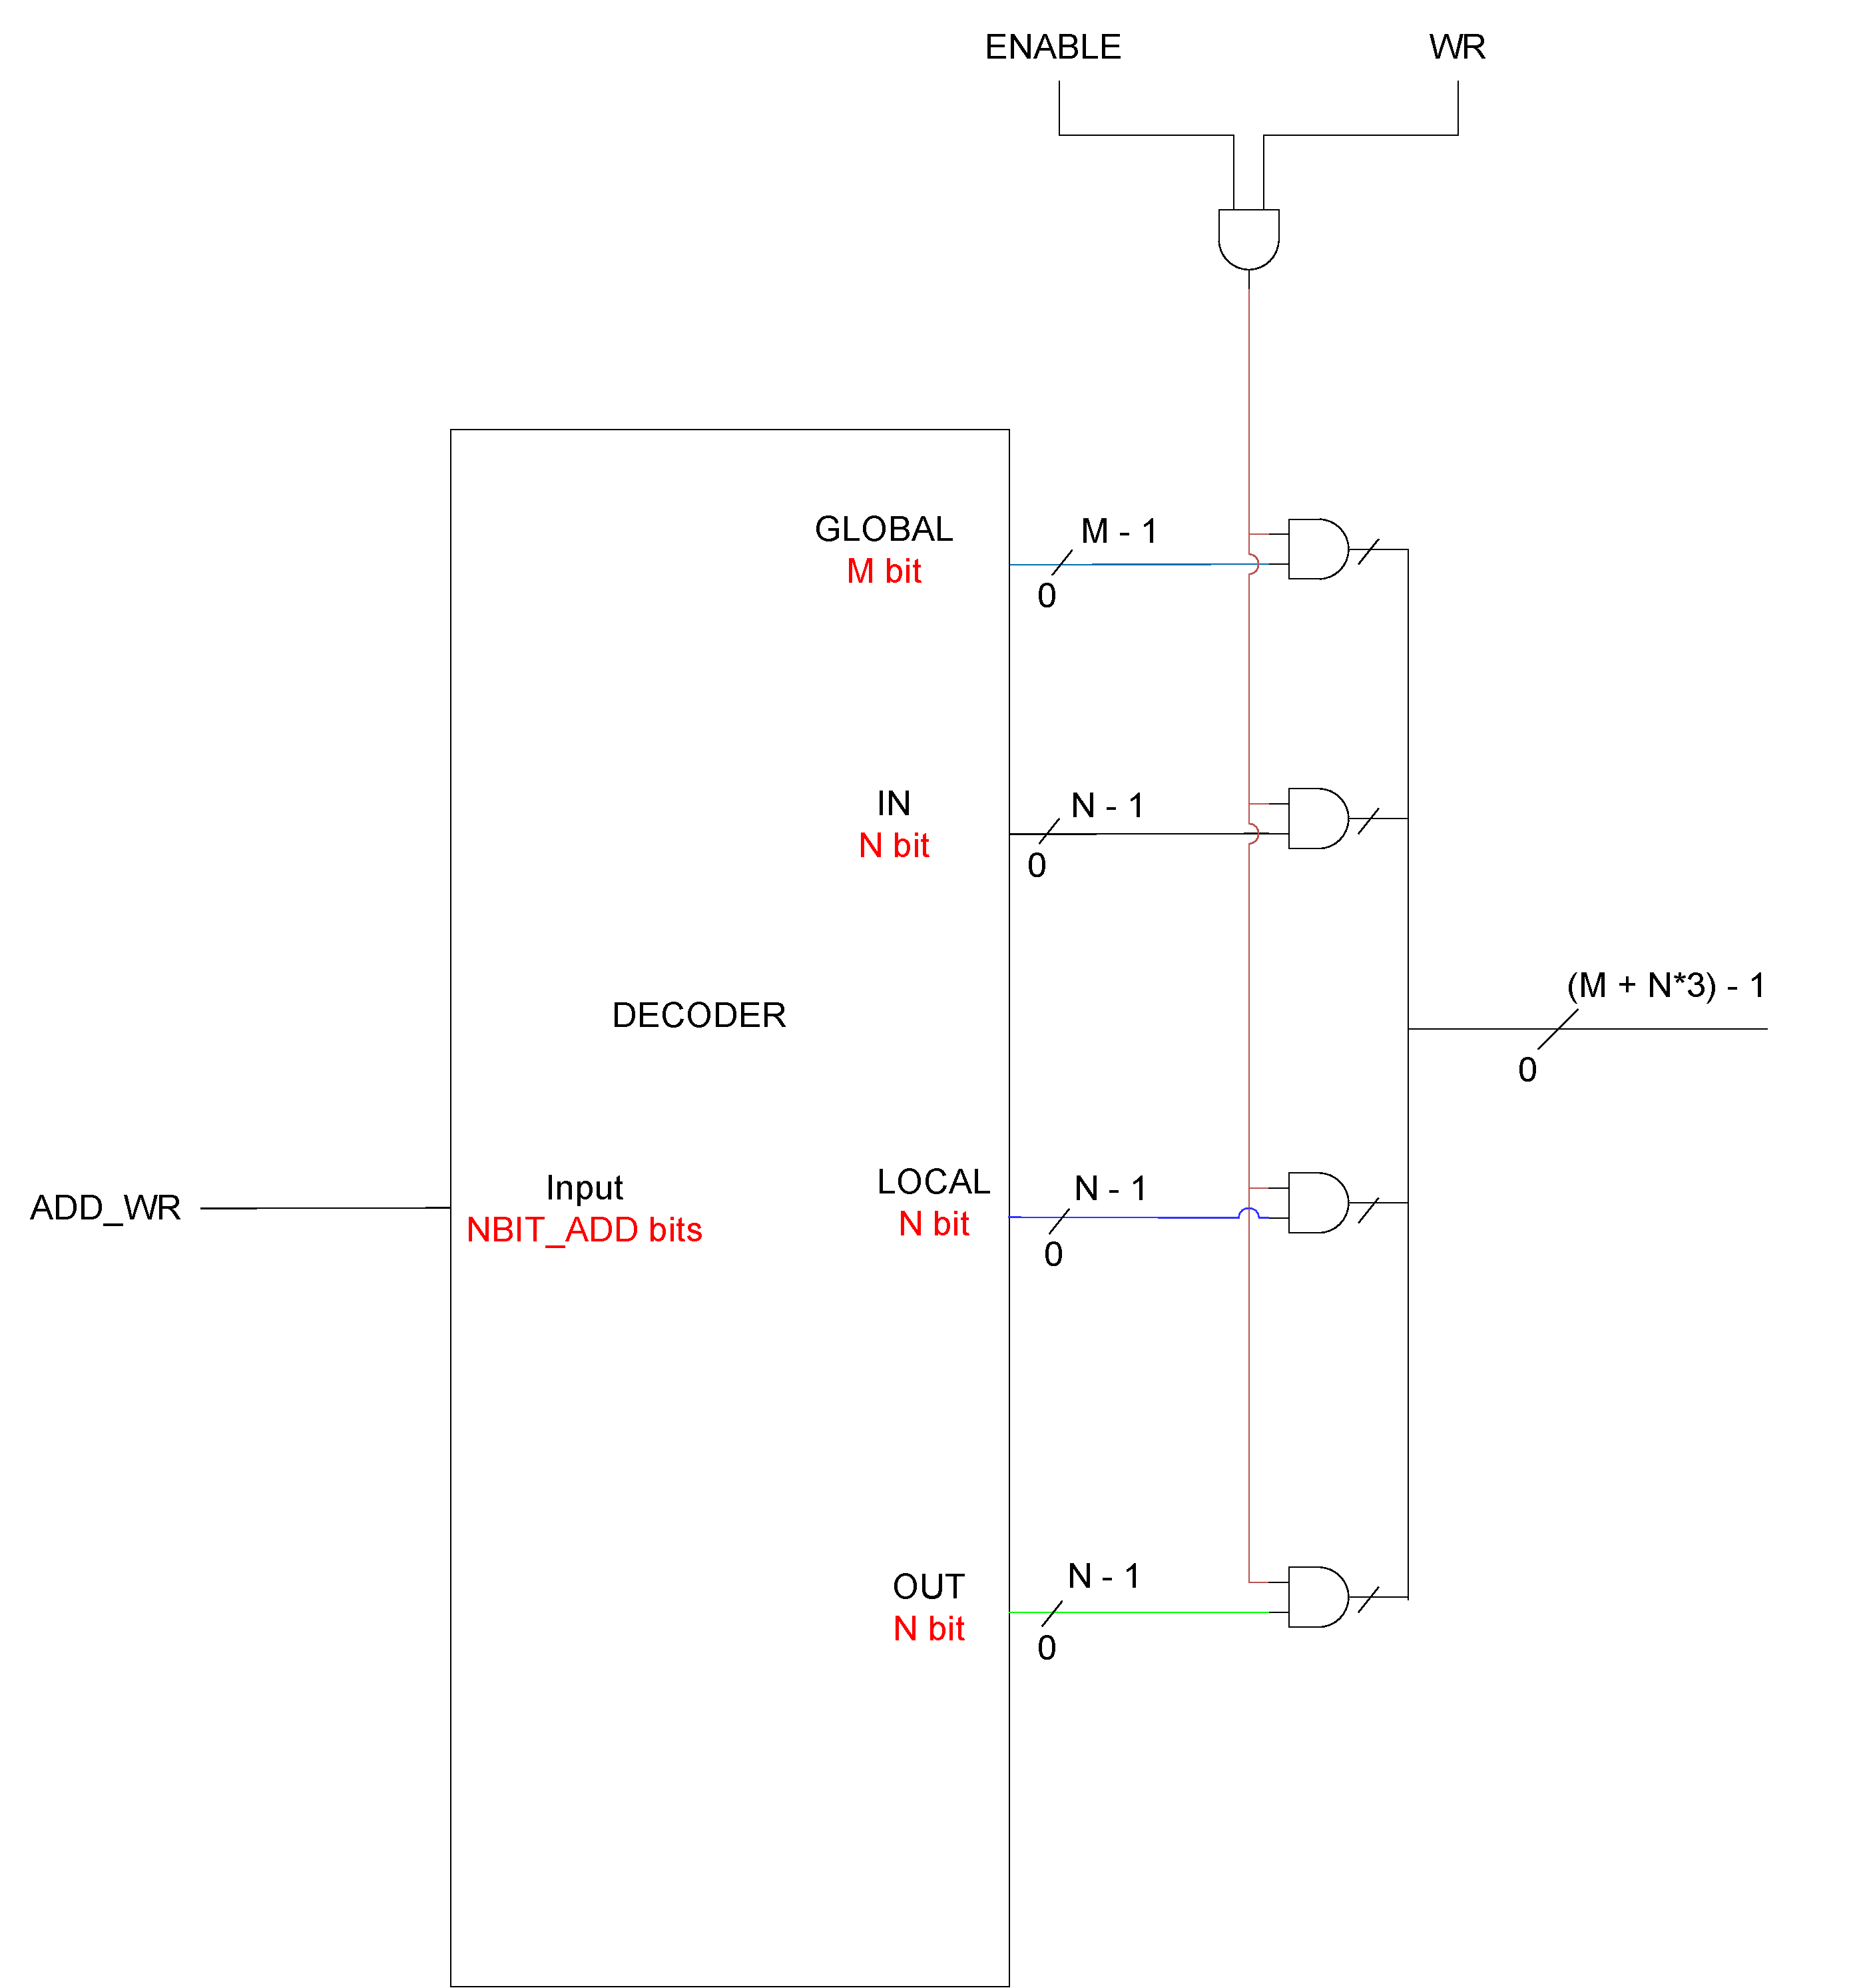
\includegraphics[width=0.7\textwidth]{Immagini/Decoder.pdf}
    \caption{Schematic of the Decoder}
    \label{decoder}
\end{figure}

\newpage
\subsection{Connection Matrix}

With the previous block, we generated all our enable signals. The problem is that we have more windows. So how do we decide which window needs to be activated? Here comes the connection matrix. This block receives as inputs the signal coming from the decoder, the current window, the saved window and the address for the pop (fill) operation. The output is a signal that contains the enable signals ready for all the registers of all windows. 

We have a specific structure for each block:
\begin{itemize}
  \item GLOBAL: the global is the simplest, because it is connected directly to the output
  \item IN: for this block we AND the IN bits coming from the decoder with the bit (that is extended) of the related window. For example if we are evaluating the IN of the first window, we will AND the IN bits with the bit 0 of the current window.
  \item OUT: for this block we AND the OUT bits coming from the decoder with the bit (that is extended) of the previous related window. For example if we are evaluating the OUT of the first window, we will AND the OUT bits with the bit 4 of the current window (supposing our window has 5 bits).
  \item LOCAL: for this block we AND the LOCAL bits coming from the decoder with the bit (that is extended) of the related window. For example if we are evaluating the LOCAL of the first window, we will AND the LOCAL bits with the bit 0 of the current window.
\end{itemize}

For the IN and OUT we then an OR between the two outputs (the logic can be seen in the schematic), while for the LOCAL we don't have anything.

In addition to that, the connection matrix also manages the saved window, used for the pop (fill) operation. First we need to invert the addr\_pop, because when we execute the pop operation, we restore data starting from the last one (we are using a STACK).
The addr\_pop\_inverted is composed like this:
\begin{itemize}
  \item 2N - 1 DOWNTO 0: we have the IN bits 
  \item N - 1 DOWNTO 0: we have the LOCAL bits
\end{itemize}

The signal is splitted into two wires and is anded with the saved related saved window pointer. 

In the end, we definitely OR the output of the previously described OR with the output of this AND. This is visible in the schematic. 


\newpage

\subsection{Register File}

The next block is the Register File, that is a sequence of registers. The important thing to notice in our design is how we managed the data that goes into the registers. We have two choice, data\_in and from\_mem. In order to choose we decided to use multiplexers. 
We have a multiplexer for each window. The signal used to drive the multiplexer is the saved window pointer, rotated right by 1 position and anded with the pop signal. In fact, we select from\_mem only when the pop signal is 1, otherwise we need to select data\_in. 
We use the saved window pointer shifted by 1 because....... TODO


\end{document}

